\documentclass[handout, dvipsnames]{beamer}
\mode<presentation>{}
\usepackage[utf8]{inputenc}
\usepackage{amsmath, amssymb, amsfonts, amsthm, mathtools, mathrsfs}
\setbeamertemplate{theorems}[numbered]
\title{Group Theory}
\author{Aryaman Maithani}
\date[23-07-2020]{23rd July 2020}
\institute[IITB]{IIT Bombay}
\usetheme{Warsaw}
% \usecolortheme{beetle}
\usepackage{graphicx}

\newcommand{\id}{\operatorname{id}}
\renewcommand{\exp}{\operatorname{exp}}

\theoremstyle{definition}
\newtheorem{defn}{Definition}
\newtheorem{prop}{Proposition}
\newtheorem{thm}{Theorem}
\begin{document}
\begin{frame}
    \titlepage
\end{frame}
\begin{frame}{Greetings}
    Hi, \uncover<2->{welcome to this }
    \begin{center}
        \uncover<3->{\emph{group}} \uncover<4->{discussion. }
    \end{center}
    \uncover<5->{Credits: Aneesh Bapat }
\end{frame}
\begin{frame}{Some examples of groups}
    \begin{itemize}
        \uncover<2->{\item The set of real numbers (/complex numbers/rational numbers) {\color<7->{red}{along with}} addition.}
        \uncover<3->{\item The set of nonzero real numbers (/complex numbers/rational numbers) {\color<7->{red}{along with}} multiplication.}
        \uncover<4->{\item The set of integers {\color<7->{red}{along with}} addition.}
        \uncover<5->{\item The set of $2\times 2$ invertible real matrices {\color<7->{red}{along with}} multiplication.}
        \uncover<6->{\item The set $\{0, 1, \ldots, n-1\}$ {\color<7->{red}{along with}} addition defined modulo $n.$}
    \end{itemize}
    \uncover<8->{Note the ``along with.'' We don't talk about a group by just talking about a set. It is necessary to have an operation on it as well.}
\end{frame}
\begin{frame}{Joke}
    \begin{center}
    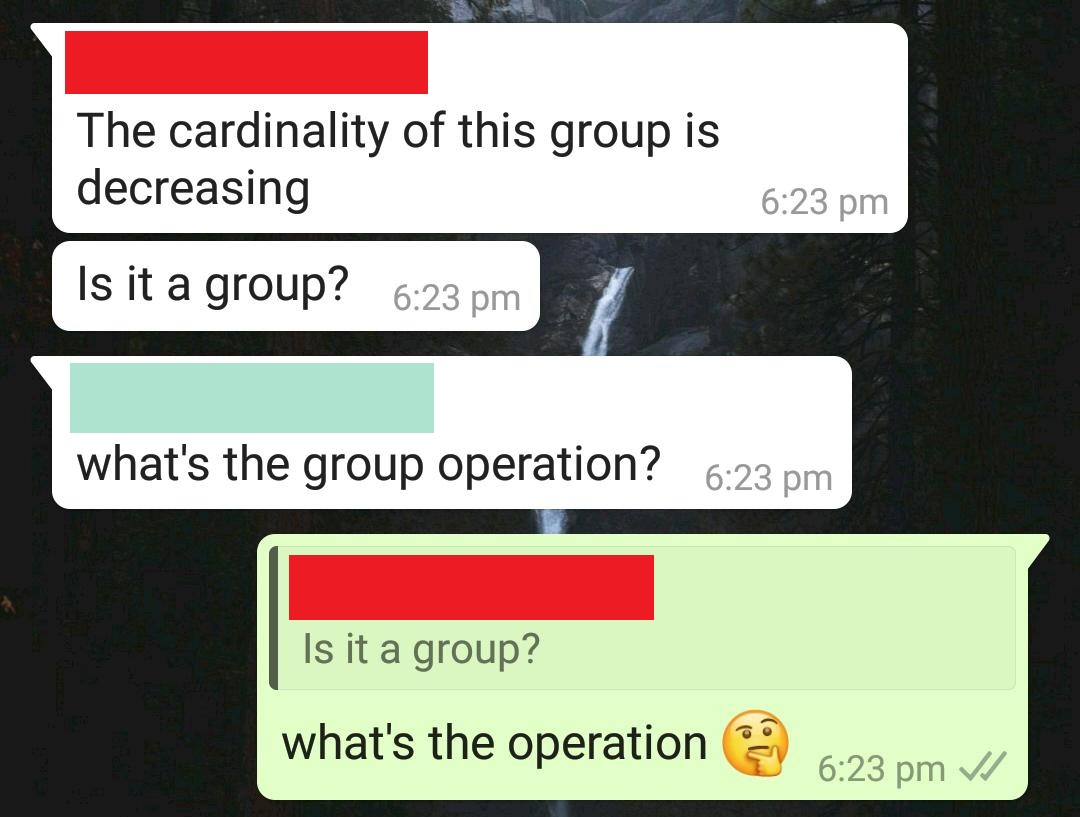
\includegraphics[width=7.5 cm]{group-operation.jpeg}
    \end{center}
\end{frame}
\begin{frame}{Some non-examples of groups}
    \begin{itemize}
        \uncover<2->{\item The set of real numbers (/complex numbers/rational numbers) along with multiplication.}
        \uncover<3->{\item The set of natural numbers along with addition.}
        \uncover<4->{\item The set of non-zero integers (/natural numbers) along with multiplication.}
        \uncover<5->{\item The set of $2\times 2$ real matrices along with multiplication.}
        \uncover<6->{\item The set $\{0, 1, \ldots, n-1\}$ with multiplication defined modulo $n.$}
        \uncover<7->{\item $\mathbb{R}^3$ with cross-product. }
        \uncover<8->{\item Empty set with the empty operation.}
    \end{itemize}
\end{frame}
\begin{frame}{What is a group?}
    \only<1|handout:0>{Hmmmmmmmmmmmmmmmmm?}
    \only<2|handout:0>{First, a definition.}
    \uncover<3->{\begin{defn}[Binary operation]
        Given a set $S,$ a binary operation $\cdot$ on $S$ is a function of the form
        \begin{equation*} 
            \cdot:S\times S \to S.
        \end{equation*}
    \end{defn}}
    \uncover<4->{For ease of notation, we shall write $a \cdot b$ instead of $\cdot\left((a, b)\right).$}\\
    \only<5|handout:0>{Examples?}
    \uncover<6->{\begin{itemize}
        \uncover<7->{\item $+$ and $\cdot$ are binary operations on $\mathbb{R}(/\mathbb{Q}/\mathbb{C}/\mathbb{Z}).$}
        \uncover<8->{\item $-$ is also a binary operation on the above sets but $\div$ is not.}
        \uncover<9->{\item $+$ is a binary operation on $\mathbb{N}$ but $-$ is not.}
        \uncover<10->{\item $+$ and $\cdot$ modulo $n$ are binary operations on $\{0, \ldots, n-1\}.$}
        \uncover<11->{\item $\times$ (cross product) is a binary operation on $\mathbb{R}^3.$}
    \end{itemize}}
    \uncover<12->{Now, we define what a group is.}
\end{frame}
\begin{frame}{What is a group?}
    \uncover<1->{\begin{defn}[Group]
        A group is an ordered pair $(G, \cdot)$ where $G$ is some set and $\cdot$ is a binary operation on $G$ satisfying the following axioms:
        \begin{enumerate}
            \uncover<2->{\item $(a \cdot b)\cdot c = a\cdot (b \cdot c)$ for all $a, b, c \in G,$}
            \uncover<3->{\item there exists an element $e$ in $G,$ called {\color<5->{red}{an}} \emph{identity} of $G,$ such that for all $a \in G$ we have $a\cdot e = a = a \cdot e,$}
            \uncover<4->{\item for each $a \in G,$ there is an element $a^{-1} \in G,$ called {\color<5->{red}{an}} \emph{inverse} of $a$ such that $a \cdot a^{-1} = e = a^{-1} \cdot a.$}
        \end{enumerate}
    \end{defn}}
    \uncover<6->{I have used ``an'' above. Why? }
    \uncover<7->{Well, simply because I can't directly claim that identity (/inverse) is unique. However, it is.}\\~\\
    \uncover<8->{\emph{Proof?}}
\end{frame}
\begin{frame}{Review}
    \only<1|handout:0>{The discussion we had is what led to us agreeing upon the above axioms. So, let us only discuss what went wrong with the non-examples.}
    \uncover<2->{\begin{itemize}
        \uncover<2->{\item The set of real numbers (/complex numbers/rational numbers) along with multiplication.}
        \uncover<3->{\item The set of natural numbers along with addition.}
        \uncover<4->{\item The set of non-zero integers (/natural numbers) along with multiplication.}
        \uncover<5->{\item The set of $2\times 2$ real matrices along with multiplication.}
        \uncover<6->{\item The set $\{0, 1, \ldots, n-1\}$ with multiplication defined modulo $n.$}
        \uncover<7->{\item $\mathbb{R}^3$ with cross-product. }
        \uncover<8->{\item Empty set with the empty operation.}
    \end{itemize}}
    \uncover<9->{Note that we need the set to be nonempty since it must always have the identity.} \\~\\
    \uncover<10->{Recall vector spaces?} \uncover<11->{Verify that any vector space along with its $+$ forms a group.}
\end{frame}
\begin{frame}{Abelian groups}
    Commutativity\uncover<2->{... is nice.}\\
    \uncover<3->{Due to this, commutative groups have a name of their own.}
    \uncover<4->{\begin{defn}[Abelian groups]
        A group $(G, \cdot)$ is said to be abelian if
        \begin{equation*} 
            a \cdot b = b \cdot a
        \end{equation*}
        for all $a, b \in G.$
    \end{defn}}
    \uncover<5->{From the second slide, everything except for the matrix example was an example of an abelian.}\\
    \uncover<6->{Even the example of $(V, +)$ for a vector space $V$ is an abelian group.} \\~\\
    \uncover<7->{{\color<8->{red}{Abel}}ian groups are named after early 19th century mathematician Niels Henrik {\color<8->{red}{Abel}}.}
\end{frame}
\begin{frame}{Abuse of notation}
    It is a common theme in math to abuse notation.\\
    \uncover<2->{Following this theme, we note that instead of writing ``$(G, \cdot)$ is a group,'' we often write the following:}
    \begin{itemize}
        \uncover<3->{\item ``$G$ is a group under $\cdot$,'' or}
        \uncover<4->{\item ``$G$ is a group'' when $\cdot$ is clear from context.}
    \end{itemize}
\end{frame}
\begin{frame}{Notations}
    Let $G$ be a group and $x \in G.$ We define $x^n$ for $n \in \mathbb{Z}$ as follows:\\~\\
    $x^0 \vcentcolon=$\uncover<2-> {$e.$}\\
    For $n > 0,$ we define
    \begin{equation*} 
        x^n \vcentcolon= \uncover<3->{\underbrace{x \cdot x \cdots  x}_{n \text{ times}}.}
    \end{equation*}
    For $n < 0,$ we have $x^n :=$\uncover<4->{$(x^{-1})^{-n}$}, which is the same as \uncover<5->{$(x^{-n})^{-1}.$} (Prove!)
    % It is convention to write $+$ as the group operation for abelian groups.
\end{frame}
\begin{frame}{Orders}
    \uncover<2->{
    \begin{defn}[Order (group)]
        The order of a group is the cardinality of $G.$\\
        It is denoted by $|G|.$
    \end{defn}}
    \uncover<3->{Note that the order of a group may be infinite. A group is said to be finite if its cardinality is.}
    \uncover<4->{\begin{defn}[Order (element)]
        The order of an element $x \in G$ the smallest positiver integer $n$ such that
        \begin{equation*} 
            x^n = e.
        \end{equation*}
        (Where $e$ is the identity of $G.$)\\
        If no such $n$ exists, then we say the the element has infinite order.\\
        It is denoted by $|x|.$
    \end{defn}
    }
\end{frame}
\begin{frame}{Finite groups}
    \begin{prop}[]
        Every element of a finite group has finite order.
    \end{prop}
    \uncover<2->{\begin{proof} 
        Let $G$ be a finite group and let $x \in G.$ \\
        It suffices to show that $x^n = e$ for \emph{some} $n \in \mathbb{N}.$\\
        Note that $x^0, x^1, \ldots, x^{|G|}$ are $|G| + 1$ elements of $G.$ By PHP, two of them must be equal. Thus,
        \begin{equation*} 
            x^n = x^m
        \end{equation*}
        for some $0 \le n < m \le |G|.$\\
        The above equation gives us
        \begin{equation*} 
            e = x^{m-n}.
        \end{equation*}
        Since $m - n \in \mathbb{N},$ we are done.
    \end{proof}}
\end{frame}
\begin{frame}{Subgroups}
    What we shall see now is a recurring theme in mathematics.\\
    \uncover<2->{Given a set with some certain properties, we look at subsets which have the same properties. }\\
    \uncover<3->{Where have you seen this before?}\\
    \uncover<4->{There are many examples:}
    \begin{itemize}
        \uncover<4->{\item Subspaces of vector spaces,}
        \uncover<5->{\item Subgroups of groups,}
        \uncover<6->{\item Subrings of rings,}
        \uncover<7->{\item Subfields of fields,}
        \uncover<8->{\item Subspaces of (metric/topological) spaces, et cetera.}
    \end{itemize}
\end{frame}
\begin{frame}{Subgroups}
    The idea is to find a subset of $G$ which can be regarded as a group in its own right. \uncover<2->{What group operation should we give it then?} \uncover<3->{Well, it is natural to consider the same operation as that of $G$.}
    \uncover<4->{\begin{defn}[Subgroup]
        A subset $H \subset G$ is said to be \emph{subgroup} of $G$ if:
        \begin{itemize}
            \uncover<5->{\item $H$ is nonempty. }
            \uncover<6->{\item $a \cdot b \in H$ for all $a, b \in H,$}
            \uncover<7->{\item $a^{-1} \in H$ for all $a \in H.$ }
        \end{itemize}
    \end{defn}}
    \uncover<8->{The above conditions just tell us that $\cdot$ (restricted to $H$) is a binary operation on $H$ and that $(H, \cdot|_H)$ forms a group. }\\~\\
    \uncover<9->{One may note that the identity element of $(G, \cdot)$ is always present in $H$ and moreover, it is also the identity of $(H, \cdot|_H).$ }
\end{frame}
\begin{frame}{Examples}
    Notation: If $H$ is a subgroup of $G,$ then we write $H \le G.$
    \begin{itemize}
        \uncover<2->{\item A group always has at least two subgroups. Can you tell which? }\uncover<3->{(Well, not two if $G$ has only one element.) }
        \uncover<3->{\item Is $\mathbb{N} \le \mathbb{Z}?$ }
        \uncover<4->{\item Is $n\mathbb{Z}\le \mathbb{Z}?$ }\uncover<5->{In fact, any subgroup of $\mathbb{Z}$ is of the form $n\mathbb{Z}$ for some $n \in \mathbb{Z}.$ }
        \uncover<6->{\item $\mathbb{Z} \le \mathbb{Q} \le \mathbb{R} \le \mathbb{C}.$ }
        \uncover<7->{\item The set of $n \times n$ invertible upper triangular (real) matrices is a subgroup of the group of all invertible $n\times n$ (real) matrices. }
    \end{itemize}
\end{frame}
\begin{frame}{Cosets}
    Let $H$ be a subgroup of $G.$ \uncover<2->{For $g \in G,$ we define $g\cdot H$ as
    \begin{equation*} 
        g\cdot H \vcentcolon= \{g\cdot h : h \in H\}.
    \end{equation*} }
    \uncover<3->{\vspace{-0.9cm}\begin{defn}[Coset]
        A \emph{(left) coset} of $H$ is a set of the form $g\cdot H.$
    \end{defn} 
    $g$ is said to be {\color{red}{a}} representative of the coset $g\cdot H.$}\\
    \uncover<4->{We define $G/H$ be the set of cosets, that is,
    \begin{equation*} 
        G/H  \vcentcolon= \{gH : g \in G\}.
    \end{equation*} }
    \uncover<5->{Note that different elements could correspond to the same coset. That is, a coset may have different representatives. }\uncover<6->{In fact, we now see precisely when that is possible. }
\end{frame}
\begin{frame}{Properties of cosets}
    \begin{prop}[Equality of cosets]
        Let $a, b \in G.$ Then, 
        \begin{equation*} 
            aH = bH \quad\text{ iff }\quad b^{-1}aH = H \quad\text{ iff }\quad b^{-1}a \in H.
        \end{equation*}
    \end{prop}
    \uncover<2->{This tells us that if $c \in aH,$ then $aH = cH.$} \uncover<3->{This also leads to the following result. }
    \uncover<4->{\begin{prop}[Disjointness of cosets]
        If $aH$ and $bH$ are two cosets, then either they are equal or they are disjoint.
    \end{prop} }
    \uncover<5->{Note that $H$ itself is a coset since it equals $e\cdot H.$ (Or $h\cdot H$ for any $h \in H.$) }
\end{frame}
\begin{frame}{Properties of cosets}
    \begin{prop}[Equality of cardinalities]
        Given any coset $aH,$ it has the same cardinality as $H.$
    \end{prop}
    \uncover<2->{(That is, there is a bijection between $aH$ and $H.$) }
    \uncover<3->{\begin{proof} 
        Consider the function $f:H \to aH$ defined by
        \begin{equation*} 
            f(h) = a\cdot h.
        \end{equation*}
        \uncover<4->{This is clearly onto, by definition of $aH.$ }\\
        \uncover<5->{Moreover, this is one-one since $ah = ah' \implies h = h'.$ }\uncover<6->{(One can cancel $a$ since it has an inverse.) }
    \end{proof} }
    \uncover<7->{\emph{Remark.} This shows that any two cosets have the same cardinality. }
\end{frame}
\begin{frame}{Lagrange's Theorem}
    \only<1|handout:0>{With the concept of cosets, we can prove a (quite fundamental) result of group theory.}
    \uncover<2->{\begin{thm}[Lagrange's Theorem]
        Let $G$ be a finite group and $H \le G.$\\
        Then, $|H|$ divides $|G|.$
    \end{thm} }
    \only<3-5|handout:0>{\begin{proof} 
        \only<4|handout:0>{\emph{Left as an exercise to the reader.}}
        \only<5|handout:0>{Jk.}
    \end{proof}}
        
    \uncover<6->{\begin{proof} 
        \uncover<6->{Consider the set of cosets $G/H = \{a_1H, \ldots, a_nH\}.$}\\
        \uncover<7->{Note that given any element $g \in G,$ it must belong to \emph{some} coset. (Why?) }\\
        \uncover<8->{Thus, $G = a_1H \cup \cdots \cup a_nH.$ }\\
        \uncover<9->{Moreover, by our previous observation, the above union is of disjoint sets. Thus, }
        \uncover<10->{
        \begin{align*} 
            |G| &= |a_1H| + \cdots + |a_nH|\\
            \uncover<11->{ &= n|H|.}
        \end{align*} }
        \uncover<12->{That completes our proof.}
    \end{proof} }
\end{frame}

\begin{frame}{Homomorphisms}
    What we consider now is another common theme in mathematics. \uncover<2->{Given two objects of the same type (for example, given two groups), we consider functions between them. }\uncover<3->{However, we don't just consider any function. We study some particular type of functions. }\\~\\
    \uncover<4->{Do you recall what particular type of functions (between vector spaces) we considered in linear algebra? }\\
    \uncover<5->{Similar to that, we consider functions that preserve the ``structure'' of the objects in consideration. }\\~\\
    \uncover<6->{The case of groups is particularly simple since there's pretty one much thing that gives the group its structure, the group operation. }\\
    \uncover<7->{This leads to the following definition. }
\end{frame}
\begin{frame}{Homomorphisms}
    \begin{defn}[Homomorphism]
        Let $(G, \cdot)$ and $(H, \star)$ be groups. A function
        \begin{equation*} 
            \varphi:G \to H
        \end{equation*}
        is said to be a \emph{group homomorphism} if
        \begin{equation*} 
            \varphi(a\cdot b) = \varphi(a)\star\varphi(b)
        \end{equation*}
        for all $a, b \in G.$
    \end{defn}
    \uncover<2->{One checks the following properties easily: }
    \begin{itemize}
        \uncover<3->{\item $\varphi(e_G) = e_H,$ }
        \uncover<4->{\item $\varphi(a^{-1}) = (\varphi(a))^{-1}$ for all $a \in G.$ }
    \end{itemize}
\end{frame}
\begin{frame}{Properties of homomorphisms}
    Now, we see some properties of homomorphisms themselves.
    \begin{itemize}
        \uncover<2->{\item Given any group $G,$ the identity function $\id_G:G\to G$ is a homomorphism from $G$ to itself. }
        \uncover<3->{\item Given homomorphisms 
        \begin{equation*} 
            G \overset{\varphi}{\longrightarrow} H \overset{\psi}{\longrightarrow} K,
        \end{equation*} the composition $\psi\circ\varphi$ is a function from $G$ to $K.$ Moreover, it is a homomorphism.\\
        \uncover<4->{Said simply: composition of homomorphisms is again a homomorphism. } }
        \uncover<5->{\item With the same notation as above, we always have
        \begin{equation*} 
            \id_H\circ \varphi = \varphi, \quad \psi\circ\id_H = \psi.
        \end{equation*} }
    \end{itemize}
    \uncover<6->{Go look up what a Category is.} \uncover<7->{(In the context of Category Theory.) }
\end{frame}
\begin{frame}{Examples}
    Let $\mathbb{R}^\times$ denote the group of nonzero real numbers under $\cdot$. Similarly, we have $\mathbb{Q}^\times$ and $\mathbb{C}^\times.$
    \begin{itemize}
        \uncover<2->{\item The map $\exp:\mathbb{R} \to \mathbb{R}^\times$ defined by 
        \begin{equation*} 
            \exp(x) = e^x
        \end{equation*} is a homomorphism because 
        \begin{equation*} 
            \exp(x + y) = e^x\cdot e^y = \exp(x)\cdot\exp(y).
        \end{equation*} }
        \uncover<3->{\item In the same way, the map $\exp:\mathbb{C} \to \mathbb{C}^\times$ is a group homomorphism. }\uncover<4->{In fact, this is surjective. }
        \uncover<5->{\item Given any $n \in \mathbb{Z},$ the map $\varphi:\mathbb{Z} \to \mathbb{Z}$ defined as
        \begin{equation*} 
            \varphi(z) = nz
        \end{equation*} is a homomorphism. }
        \uncover<6->{\item In general, if $G$ is an abelian group and $n \in \mathbb{Z},$ the map $x \mapsto x^n$ is a homomorphism. }
    \end{itemize}
\end{frame}
\begin{frame}{Isomorphisms}
    Homomorphisms lead to another equally recurring concept in mathematics. \uncover<2->{The concept of isomorphism. }\uncover<3->{Loosely speaking, an isomorphism captures two structures to be ``equivalent.'' }\\~\\
    \uncover<4->{For example, consider the group $\{0, 1, 2\}$ with addition modulo $3$ and the group $\{1, \omega, \omega^2\}$ with multiplication. ($\omega = \exp\left(\frac{2\pi}{3}i\right).$) }\\~\\
    \uncover<5->{While the groups are not equal (since they don't have the same element), they pretty much are same in terms of the group properties. }\\
    \uncover<6->{This idea can formalised as follows. }
\end{frame}
\begin{frame}{Isomorphisms}
    \begin{defn}[Isomorphism]
        Let $G$ and $H$ be groups. A group homomorphism $\varphi:G \to H$ is said to be an \emph{isomorphism} if $\varphi$ is bijective.
    \end{defn}
    \uncover<2->{\emph{Remark.} It can be checked that the inverse of a bijective homomorphism is again a homomorphism.} \uncover<3->{In particular, if $\varphi$ is an isomorphism, then so is $\varphi^{-1}.$ }\\
    \uncover<4->{\begin{defn}[Isomorphic]
        Two groups $G$ and $H$ are said to be isomorphic if there exists a group isomorphism $\varphi:G \to H.$\\
        In such a case, we write $G \cong H.$
    \end{defn} }
    \uncover<5->{One can note that $\cong$ is an ``equivalence relation''. }

\end{frame}
\begin{frame}{Examples}
    \begin{itemize}
        \uncover<2->{\item With $G = \{0, 1, 2\}$ and $H = \{1, \omega, \omega^2\}$ as earlier, we see that $\varphi:G\to H$ defined by $\varphi(i) = \omega^i$ is an isomorphism. }
        \uncover<3->{\item In general, the groups $G = \{0, \ldots, n-1\}$ and $H = \{z \in \mathbb{C}^\times : z^n = 1\}$ are isomorphic. }
        \uncover<4->{\item The map $\exp:\mathbb{R} \to \mathbb{R}^+$ is an isomorphism. (Note that $\mathbb{R}$ is a group under $+$ whereas $\mathbb{R}^+$ is a group under $\cdot$.) }
    \end{itemize}
\end{frame}

\begin{frame}{Kernels}
    Once again, let us look at a concept the quite recurring in mathematics. (This time more focused in the realm of algebra.)
    \uncover<2->{\begin{defn}[Kernel]
        Given a group homomorphism $\varphi:G \to H,$ we denote the \emph{kernel} of $\varphi$ by $\ker \varphi$ and define it as
        \begin{equation*} 
            \ker\varphi \vcentcolon= \{g \in G : \varphi(g) = e_H\}.
        \end{equation*}
    \end{defn} }
    \uncover<3->{That is, it is the subset of $G$ consisting of all those elements that get mapped to the identity of $H.$ }\uncover<4->{Does this remind you of anything from linear algebra? }
    \uncover<5->{\begin{prop}[]
        With the same notations as above, we have 
        \begin{equation*} 
            \ker \varphi \le G.
        \end{equation*}
    \end{prop} }
\end{frame}
\begin{frame}{A curious property about kernels}
    \begin{prop}[]
        Let $\varphi:G \to H$ and $K = \ker\varphi.$\\
        Then, given any $a \in G$ and $k \in K,$ we have
        \begin{equation*} 
            aka^{-1} \in K.
        \end{equation*}
    \end{prop}
    \uncover<2->{The above says that $aKa^{-1} \subset K$}\uncover<3->{, where $aKa^{-1}$ is defined in the natural manner as
    \begin{equation*} 
        \{aka^{-1} : k \in K\}.
    \end{equation*} }\\
    \uncover<4->{In fact, since the above is true for all $a \in G,$ it is also true for $a^{-1}$ and we actually get the equality $aKa^{-1} = K.$ }\\~\\
    \uncover<5->{This can be written in yet another way as ${\color{orange}{aK = Ka}}.$ }
\end{frame}
\begin{frame}{A curious calculation}
    Now, suppose that ${\color{red}a}, {\color{red}a'}, {\color{blue}b}, {\color{blue}b'} \in G$ are elements such that ${\color{red}a}K = {\color{red}a'}K$ and ${\color{blue}b}K = {\color{blue}b'}K.$\\
    \uncover<2->{Then, we see that }
    \begin{align*} 
        \uncover<3->{({\color{red}a}{\color{blue}b})K &= a({\color{blue}b}K)}\\
        \uncover<4->{&= {\color{red}a}(K{\color{blue}b}) }\\
        \uncover<5->{&= {\color{red}a}(K{\color{blue}b'}) }\\
        \uncover<6->{&= ({\color{red}a}K){\color{blue}b'} }\\
        \uncover<7->{&= ({\color{red}a'}K){\color{blue}b'} }\\
        \uncover<8->{&= {\color{red}a'}(K{\color{blue}b'}) }\\
        \uncover<9->{&= ({\color{red}a'}{\color{blue}b'})K.}
    \end{align*}
    \uncover<10->{Let us keep this in mind for now. We shall come back to it later.}\\
    \uncover<11->{Note that the only property we used was that ${\color{orange}{gK = Kg}}$ and not really that $K$ was a kernel. }
\end{frame}
\begin{frame}{Coming back to cosets}
    Recall the set of cosets $G/H.$ \uncover<2->{We wish to turn this set into a group.}\\~\\
    \uncover<3->{What should the group operation be? }\\
    \uncover<4->{Well, given cosets $aH$ and $bH,$ we wish to define $(aH)(bH).$ }\\
    \uncover<5->{Moreover, the product must again be a coset. }\\~\\
    \uncover<6->{So, the question is: What $g \in G$ should be pick to define
    \begin{equation*} 
        (aH)(bH) = gH?
    \end{equation*} }
    \uncover<7->{Well, the natural choice is: $g = ab.$ }\\
    \uncover<8->{However, there is a problem... }
\end{frame}
\begin{frame}{A problem :(}
    When we talk about the product $(aH)(bH),$ we are defining products of two \emph{sets}.\\
    \uncover<2->{Now, given any coset of $H,$ it is true that it can be written as $aH$ for \emph{some} $a \in G.$ }\\
    \uncover<3->{However, the problem is that the $a$ is not (always) unique. }\\
    \uncover<4->{Thus, when defining the product, the product must not depend on the representative chosen. }\\
    \uncover<5->{This means that we must take care of the following: }\\~\\
    \uncover<6->{Whenever we have ${\color{red}a}H = {\color{red}a'}H$ and ${\color{blue}b}H = {\color{blue}b'}H$}\uncover<7->{, we must have
    \begin{equation*} 
        \only<7-8|handout:0>{ ({\color{red}a}H)({\color{blue}b}H)}%
        \only<8>{=}\uncover<8-9>{({\color{red}a}{\color{blue}b})H = ({\color{red}a'}{\color{blue}b'})H}%
        \only<7-8|handout:0>{= ({\color{red}a'}H)({\color{blue}b'}H)}.
    \end{equation*} }
\end{frame}
\begin{frame}{Solving the problem :)}
    \uncover<1->{Well, what does that remind us of?} \uncover<2->{That was a property kernels of homomorphisms have! }\\
    \uncover<3->{In fact, what we saw was that all we need is that ${\color{orange}{gH = Hg}}$ (for all $g \in G$) and then, we always have the desired property. }\\~\\
    \uncover<4->{Note that we have shown that if ${\color{orange}{gH = Hg}},$ then the multiplication is well-defined. }\\
    \uncover<5->{In fact, the converse is true as well.} \uncover<6->{That is,} \uncover<7->{if
    \begin{equation*} 
        {\color{red}a}H = {\color{red}a'}H, {\color{blue}b}H = {\color{blue}b'}H \implies ({\color{red}a}{\color{blue}b})H = ({\color{red}a'}{\color{blue}b'})H,
    \end{equation*}} 
    \uncover<8->{then $H$ must satisfy ${\color{orange}{gH = Hg}}.$ }
\end{frame}
\begin{frame}{Normal subgroups}
    The previous discussion brings us to an important notion - that of a \emph{normal} subgroup. \uncover<2->{What do you think is the definition? }
    \uncover<2->{\begin{defn}[Normal subgroup]
        \uncover<2->{A subgroup $N$ of a group $G$ is said to be \emph{normal} if }
        \uncover<3->{
        \begin{equation*} 
            gN = Ng
        \end{equation*}
        for all $g \in G.$ }
    \end{defn} }
    \uncover<4->{Said differently, we must have $gNg^{-1} = N$ for all $g \in G.$ }\\
    \uncover<5->{Said even more differently, given any $n \in N,$ and $g \in G,$ we must have $gng^{-1} \in N.$ }
\end{frame}
\begin{frame}{Quotienting}
    With this, we come to the last theme for today, another very recurring theme in mathematics \uncover<2->{- \emph{quotienting}. }\\
    \only<3|handout:0>{We first look at the definition and then have discussion about the theme. }
    \uncover<4->{\begin{defn}[Quotient group]
        Let $G$ be a group and $N$ be a normal subgroup of $G.$\\
        Then, the set of cosets $G/N$ is a group under the operation defined by
        \begin{equation*} 
            (aN)(bN) \vcentcolon= (ab)N,
        \end{equation*}
        which is well-defined in view of our previous discussion.
    \end{defn} }
    \uncover<5->{We sometimes use the notation $\bar{g}$ to denote the coset $gH.$ (When $H$ is clear from context.) }\\
    \uncover<6->{Another thing to note is that any subgroup of an abelian group is normal. }
\end{frame}
\begin{frame}{Example}
    Consider the group $(\mathbb{Z}, +)$ and the subgroup ${\color{ProcessBlue}5}\mathbb{Z}.$ (Is this normal?)\\
    \uncover<2->{(Since the group operation is denoted with $+,$ we will use $+$ to denote the cosets as well.) }\\
    \uncover<3->{As an example, one of the cosets of ${\color{ProcessBlue}5}\mathbb{Z}$ is 
    \begin{equation*} 
        2 + {\color{ProcessBlue}5}\mathbb{Z} = \{\ldots, -8, -3, 2, 7, 12, \ldots\}.
    \end{equation*} }
    \uncover<4->{The set of cosets is $\{\bar{0}, \bar{1}, \bar{2}, \bar{3}, \bar{4}\}.$ }\uncover<5->{The addition (as an example) is like 
    \begin{equation*} 
        \bar{1} + \bar{2} = \bar{3}, \quad \bar{3} + \bar{4} = \bar{2}, \quad \bar{2} + \bar{3} = \bar{0}.
    \end{equation*} }
    \uncover<6->{Basically, this is just addition modulo ${\color{ProcessBlue}5}.$ }\\~\\
    \uncover<7->{The above group is what is called $\mathbb{Z}/{\color{ProcessBlue}5}\mathbb{Z}.$ }\uncover<8->{Of course, this works for all values of ${\color{ProcessBlue}5}.$ }\\
    \uncover<9->{In fact, this is the group (up to isomorphism) which we saw earlier as $\{1, \ldots, {\color{ProcessBlue}n}-1\}$ with addition modulo ${\color{ProcessBlue}n}.$ }
\end{frame}
\begin{frame}{Exercises}
    1. Let $(G, \cdot)$ be a finite group and let $x \in G.$\\
    Show that $H = \{1, x, x^2, \ldots\}$ is a (finite) subgroup of $G.$\\~\\
    Show that $H$ has order $|x|.$\\~\\
    Conclude that $|x|$ divides $|G|.$ \\
    In particular, we have $x^{|G|} = e.$
\end{frame}
    
\begin{frame}{Exercises}
    2. Let $n > 1$ be a natural number. Define
    \begin{equation*} 
        (\mathbb{Z}/n\mathbb{Z})^* = \{x : 1 \le x \le n, \gcd(x, n) = 1\}.
    \end{equation*}
    Show that $|(\mathbb{Z}/n\mathbb{Z})^*| = \varphi(n),$ where $\varphi$ is the Euler totient function.\\~\\
    Show that $(\mathbb{Z}/n\mathbb{Z})^*$ is a group under the operation ``multiplication mod $n$'' with identity being $1.$\\~\\
    Conclude that $a^{\varphi(n)} = 1$ for all $a \in (\mathbb{Z}/n\mathbb{Z})^*.$ (Note that this equality is in the group $(\mathbb{Z}/n\mathbb{Z})^*.$)\\~\\
    Conclude that $a^{\varphi(n)} \equiv 1 \bmod n$ for all $a$ with $\gcd(a, n) = 1.$\\~\\
    This is Euler's theorem (in number theory) and Fermat's little theorem is a special case of it.
\end{frame}

\begin{frame}{Exercises}
    3. Let $G$ be a finite group and let $p$ be a prime dividing $|G|.$ Let $\mathcal{S}$ denote the set of $p$-tuples of elements of $G$ the product of whose coordinates is $1:$
    \begin{equation*} 
        \mathcal{S} = \{(x_1, \ldots, x_p) : x_i \in G \text{ and } x_1x_2\cdots x_p = 1\}.
    \end{equation*}
        (a) Show that $\mathcal{S}$ has $|G|^{p-1}$ elements, hence has order divisible by $p.$\\~\\
        Define the relation $\sim$ on $\mathcal{S}$ be letting $\alpha \sim \beta$ if $\beta$ is a cyclic permutation of $\alpha.$\\~\\
        (b) Show that a cyclic permutation of an element of $\mathcal{S}$ is again an element of $\mathcal{S}.$ \\
        (c) Prove that $\sim$ is an equivalence relation on $\mathcal{S}.$\\
        (d) Prove that an equivalence class contains a single element if and only if it is of the form $(x, \ldots, x)$ with $x^p = 1.$\\
\end{frame}
\begin{frame}{Exercises}
        (e) Prove that every equivalence class has order $1$ or $p$ (this uses the fact that $p$ is a \emph{prime}). Deduce that $|G|^{p-1} = k + pd$ where $k$ is the number of classes of size $1$ and $d$ is the number of classes of size $p.$\\
        (f) Since $\{(1, \ldots, 1)\}$ is an equivalence class of size $1,$ conclude from (e) that there must be a nonidentity element $x$ in $G$ with $x^p = 1,$ i.e., $G$ contains an element of order $P.$ (Show $p \mid k$ and so $k > 1.$)
\end{frame}
\begin{frame}{}
    The previous exercise proves the following theorem.
    \begin{thm}[Cauchy's Theorem]
        If $G$ is a finite group and $p \mid |G|,$ then there exists $x \in G$ such that $p = |x|.$
    \end{thm}
    With $H = \{1, x, \ldots\}$ as in Exercise 1, this shows that there exists a subgroup of order $p.$ \\
    This is a partial converse to Lagrange's theorem (and the statement shown in Exercise 1). \\
    (And that's the best we can get.) \\~\\
    \emph{Credits:} The above style of proof was published in Amer. Math. Monthly, 66 (1959), p. 199 by James McKay.\\
    The above exercise has been taken from Abstract Algebra by Dummit and Foote.
\end{frame}
\begin{frame}{Exercises}
    4. Let $n \ge 1$ be a natural number and define 
    \begin{equation*} 
        [n] = \{1, \ldots, n\}.
    \end{equation*}
    Let $S_n$ denote the set of all \emph{bijections} from $[n]$ to $[n].$\\
    Let $\circ$ denote the usual composition operation of functions.\\~\\
    (a) Show that $\circ$ is a binary operation on $S_n.$\\
    (b) Show that $S_n$ is a group under $\circ.$\\
    This is known as the \emph{symmetric group} on $n$ elements.\\
    This is a very common example of a (family of) group.\\
    (c) Show that $S_n$ is abelian if and only if $n \le 2.$\\~\\
    A remarkable theorem called \emph{Cayley's theorem} says that any (finite) group is isomorphic to a subgroup of $S_n$ for some $n.$
\end{frame}
\end{document}
% 5025396551